\subsection{Experiment}
\begin{comment}
\begin{figure}
% We need layers to draw the block diagram
\pgfdeclarelayer{background}
\pgfdeclarelayer{foreground}
\pgfsetlayers{background,main,foreground}

% Define a few styles and constants
\tikzstyle{sensor}=[draw, fill=blue!20, text width=5em,text centered, minimum height=2.5em]
\tikzstyle{system} = [sensor, text width=6em, fill=green!30, 
    minimum height=12em, rounded corners]
\tikzstyle{input} = [coordinate]
\tikzstyle{sum} = [draw, fill=blue!20, circle, node distance=1cm]
%\tikzstyle{output} = [coordinate]
\def\blockdist{0.5}
\def\edgedist{0.75}
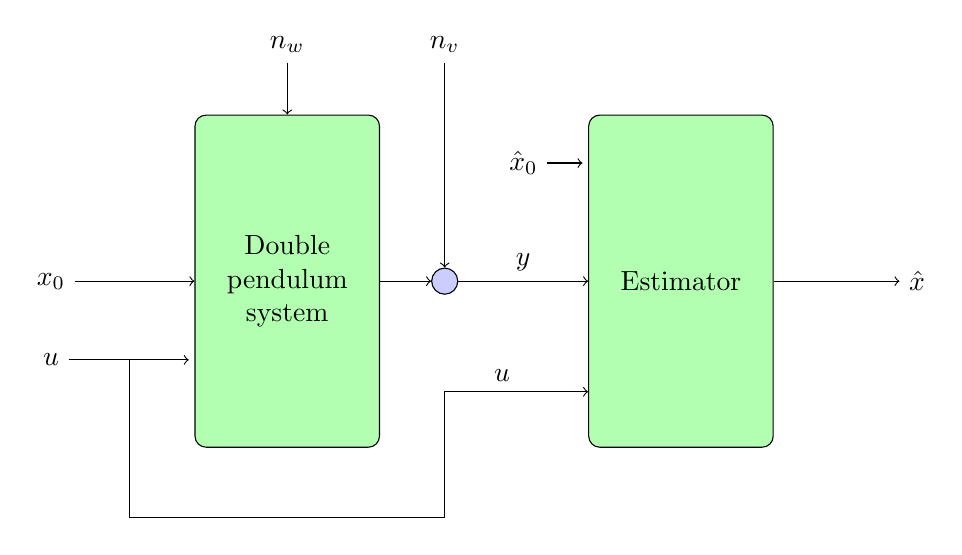
\begin{tikzpicture}
	% Define the nodes in the picture
	\node (sys_in)[yshift=1cm]{$x_0$};
	\node (u_in) [below of=sys_in,node distance=1cm]{$u$};
	\node (sys_u)[input,right of=u_in,node distance=1cm]{};
    \node (sim_sys) [system,right of=sys_in,node distance=3cm] {Double pendulum system};
    \node (sys_noise)[above of=sim_sys,node distance=3cm]{$n_w$};
    \node (msr_noise)[right of=sys_noise,node distance=2cm]{$n_v$};
    \node (msr_add)[sum,right of=sim_sys,node distance=2cm]{};
    \node (estimator) [system,right of=msr_add,node distance =3cm]{ Estimator};
    \node (est_in) [right of=sim_sys,node distance=3cm,yshift=1.5cm]{$\hat{x}_0$};
    \node (est_u) [input,right of =sim_sys, node distance=2cm,yshift=-3cm]{foo};
    \node (est_out)[right of=estimator,node distance=3cm]{$\hat{x}$};
    
    % Define the edges in the picture
    \draw [->] (sys_in) --node{}(sim_sys.west);
    \draw [-] (u_in) --node{}(sys_u);
    \draw [->] (sys_u) --node{}+(\edgedist,0);
    \draw [-] (sys_u) |-node{}(est_u);
    \draw [->] (est_u) |-node[pos=0.7,above]{$u$}(estimator.-130);
    \draw [->] (est_in) --node{}+(\edgedist,0);
    \draw [->] (sys_noise) --node{}(sim_sys.north);
    \draw [->] (msr_noise) --node{}(msr_add.north);
    \draw [->] (sim_sys.east) --node[above]{}(msr_add.west);
    \draw [->] (msr_add.east) --node[above]{$y$}(estimator.west);
    \draw [->] (estimator) --node{}(est_out);
\end{tikzpicture}
\caption{Experimental setup for the simple model}
\end{figure}
\end{comment}

The experimental setup shown in Figure \ref{fig:toro_exp} is used for testing the EKF. An IMU that outputs the accelerations $a$ and angular velocity $\omega$ with respect to the body reference frame is simulated by the simulator. For instance when the IMU is attached to the hip (floating base), its outputs are defined with respect to the hip reference frame. The biases $b_a,b_\omega$ and noises $w_a,w_\omega$ are externally added to the IMU outputs. The following scenario is considered for this experiment. 

The same experimental scenario described in \ref{subsec:toro_exp} is used for testing the EKF. The following noise and bias values are used in simulations:

\begin{table}
	\centering
	\begin{tabular}{|c|c|}
	\hline
	Name of the sensor &Noise variance \\ \hline
	Accelerometer ($w_a$) & $8 \cdot {10}^{-3}$ \\
	Gyroscope ($w_\omega$) & $5 \cdot {10}^{-3}$ \\ \hline	
	\end{tabular}
	\caption{Variances of sensor noise used in simulation}
	\label{tab:simp_noise}
\end{table}

The hand tuned values of process noise covariance matrix $Q$ is 
$$ Q = diag([ 1 \cdot {10}^{-3} \textbf{1}_{3,1}, 1 \cdot {10}^{-8} \textbf{1}_{3,1}, 1 \cdot {10}^{-15} \textbf{1}_{6,1}]). $$
The contact measurements are highly accurate. The hand tuned values of measurement covariance matrix $R$ is $$R = diag(1 \cdot {10}^{-12} \textbf{1}_{24,1}).$$

\subsubsection{Observation}
\begin{figure}
    \centering
    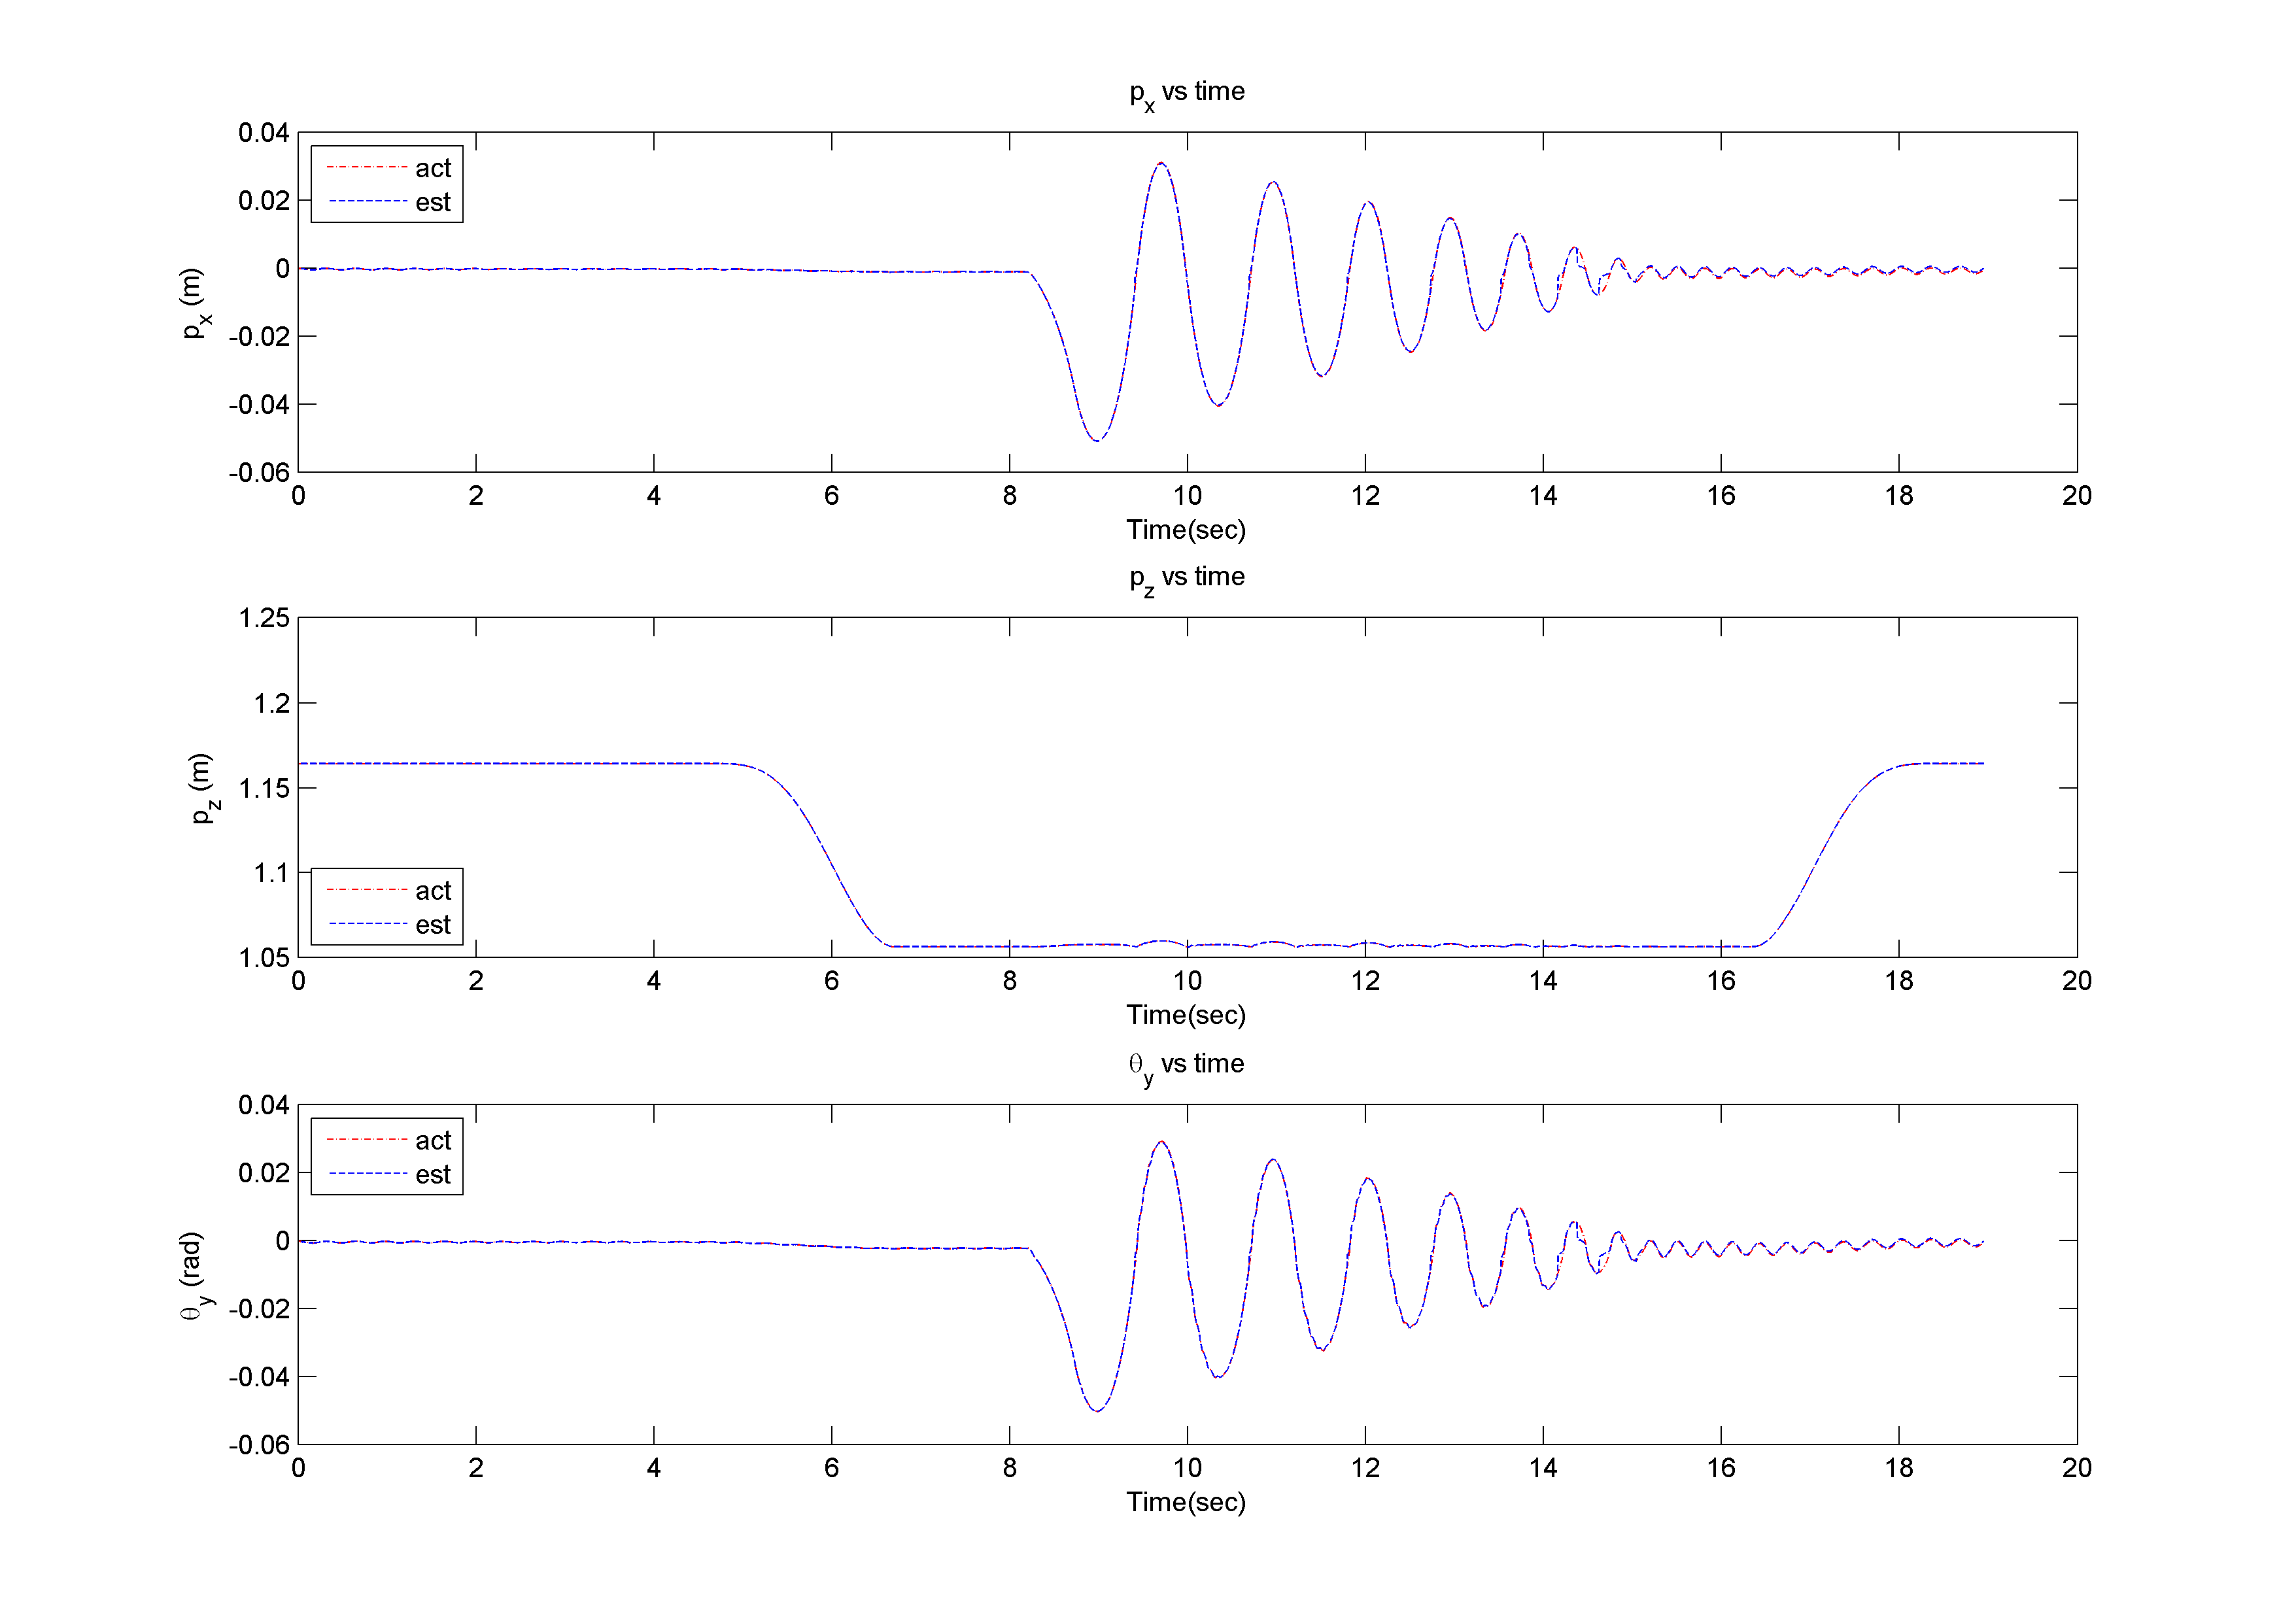
\includegraphics[trim=20mm 10mm 25mm 10mm,clip,scale=0.55]{Bilder/plots/simple_model/pos.png}
    \caption{Actual and estimated values of $p_x,p_z$ and $\theta_y$}
    \label{fig:simp_plotpos}
\end{figure}
\begin{figure}
    \centering
    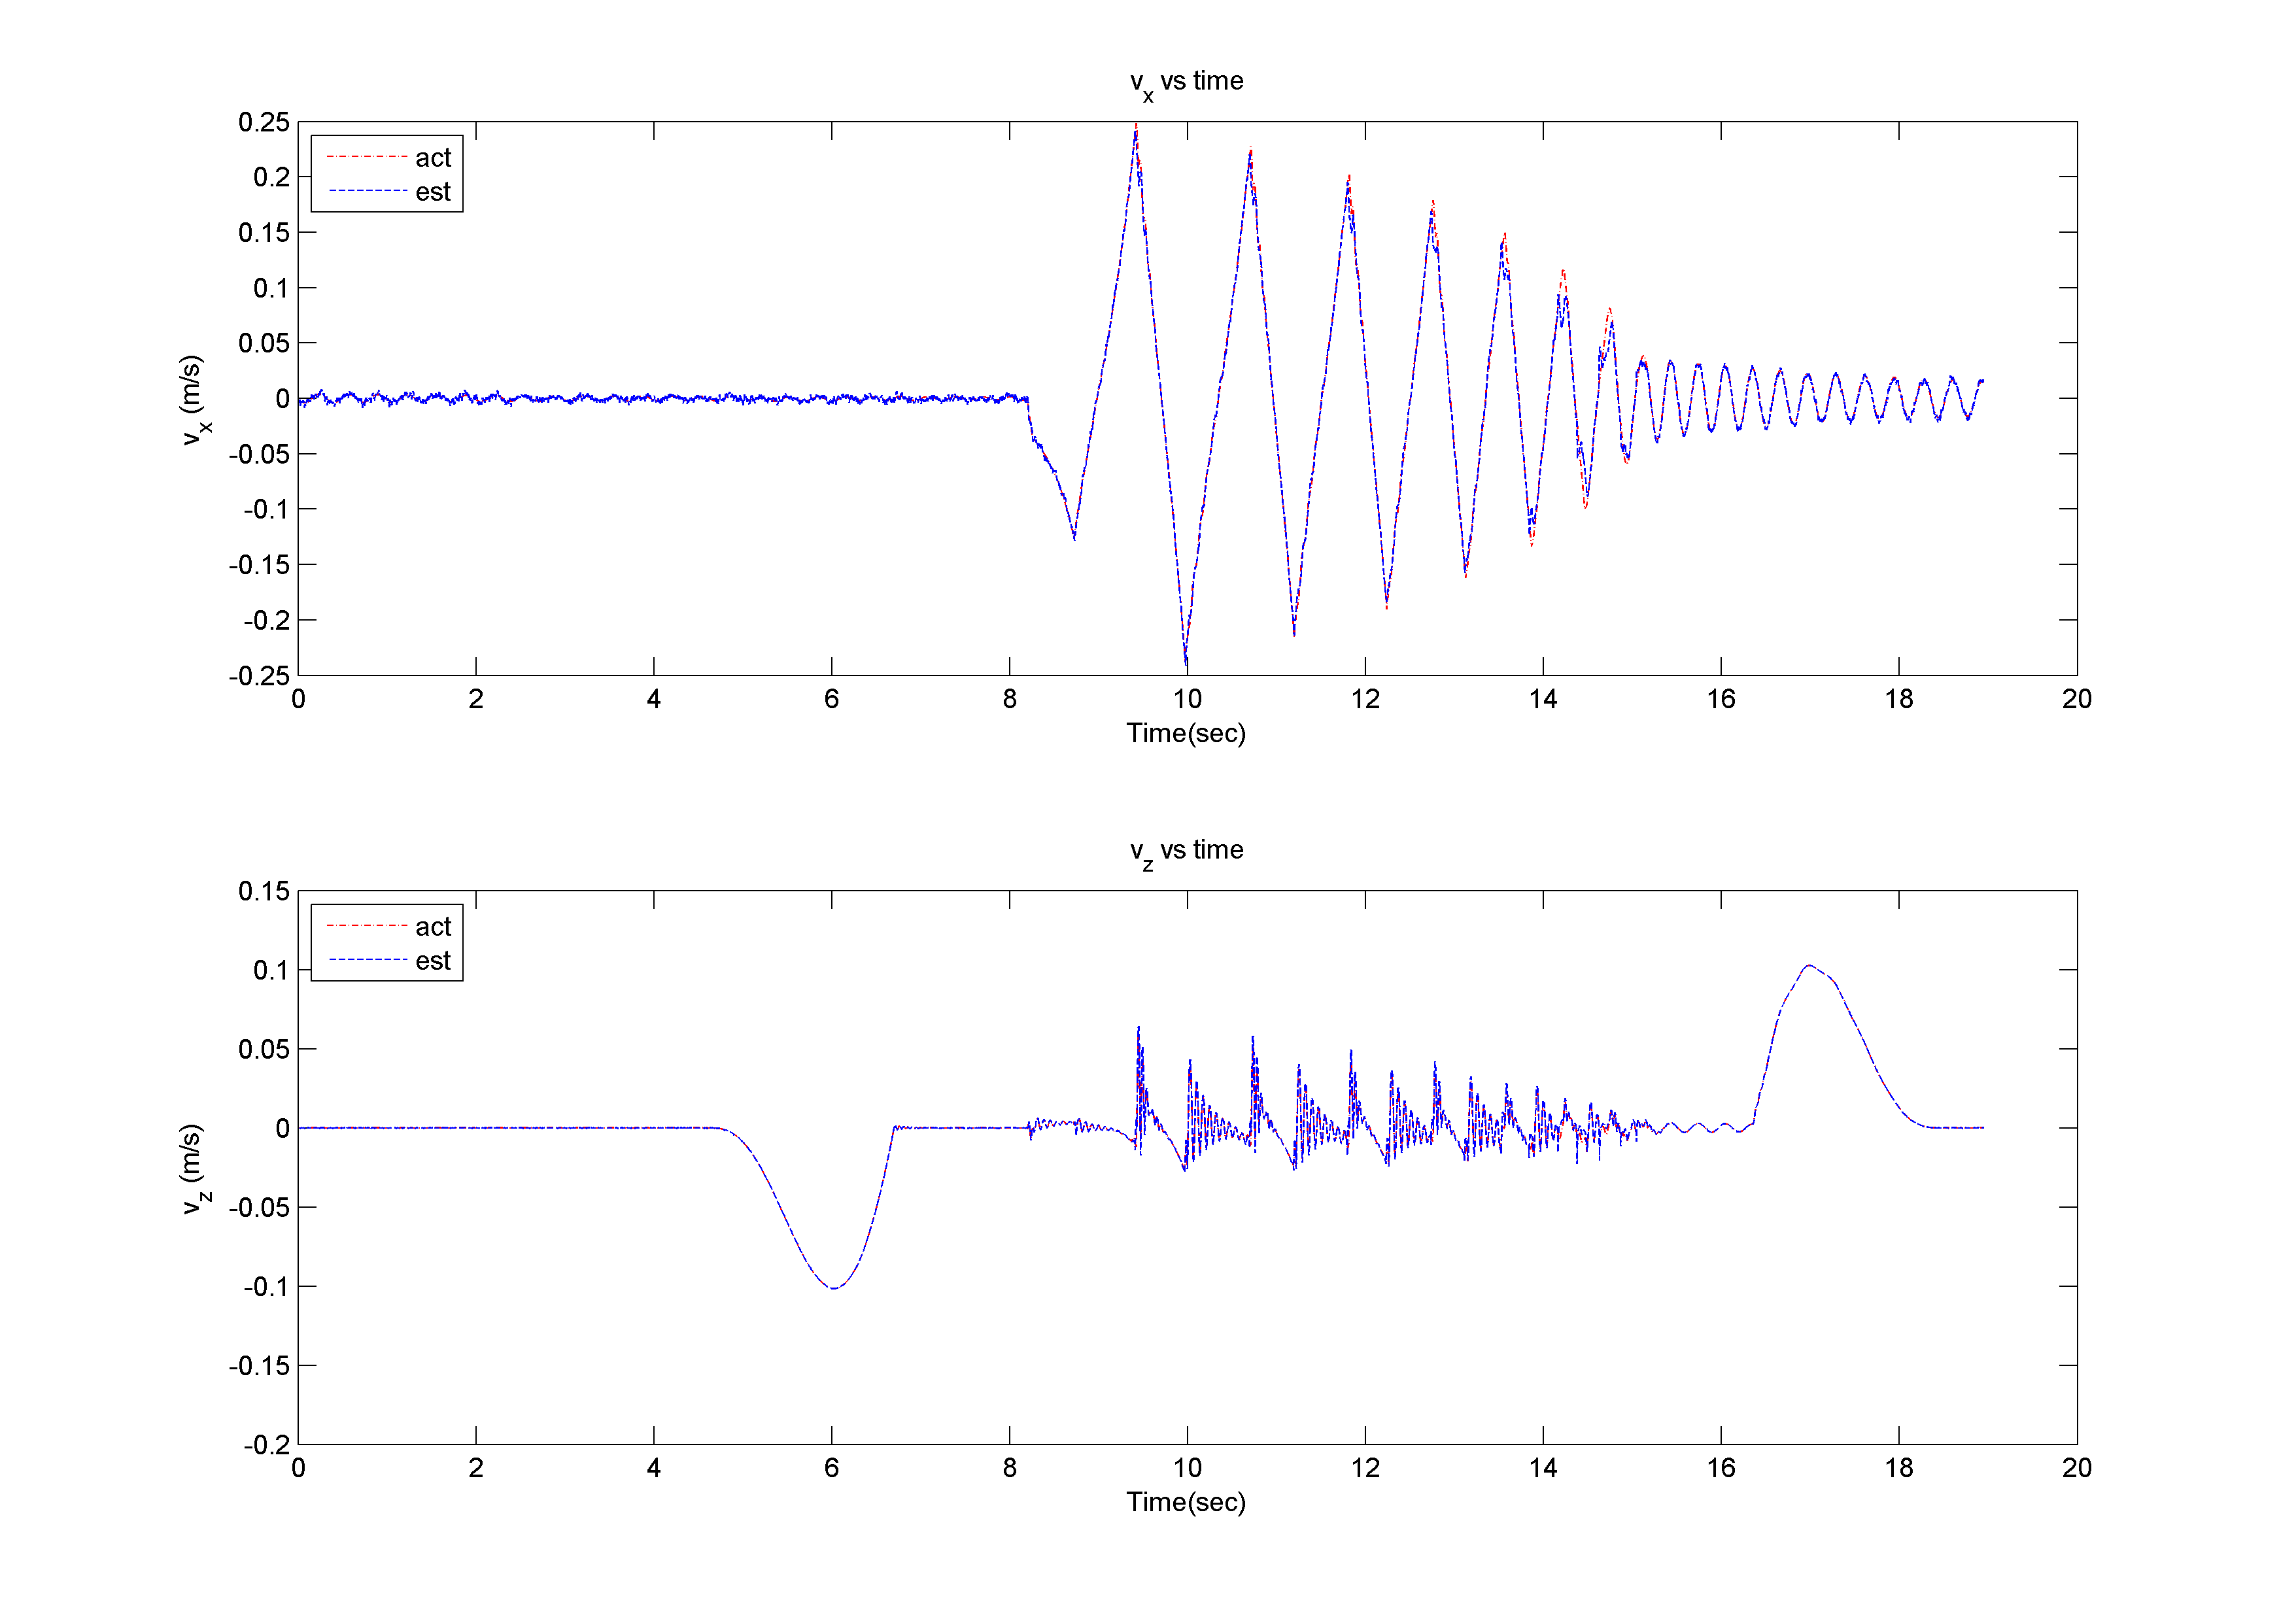
\includegraphics[trim=20mm 10mm 25mm 10mm,clip,scale=0.55]{Bilder/plots/simple_model/vel.png}
    \caption{Actual and estimated values of $v_x$ and $v_z$}
    \label{fig:simp_plotvel}
\end{figure}
It can be seen in the Figures \ref{fig:simp_plotpos} and \ref{fig:simp_plotvel} the estimates follows the actual states. 
\begin{table}
    \centering
    \begin{tabular}{|c|c|}
    \hline
    Estimates &RMSE \\ \hline
    $\hat p_x$ &0.0005 $m$\\
    $\hat p_y$ &0.0001 $m$\\
    $\hat p_z$ &0.0002 $m$\\
    $\hat\theta_x$ &0.0001 $rad$\\
    $\hat\theta_y$ &0.0005 $rad$\\
    $\hat\theta_z$ &0.0003 $rad$\\ 
    $\hat v_x$ &0.0051 $m/s$\\
    $\hat v_y$ &0.0018 $m/s$\\
    $\hat v_z$ &0.0090 $m/s$\\\hline
    \end{tabular} \hspace{1cm}
    \caption{RMSE values of position and velocity estimates}
    \label{tab:simp_rmse}
\end{table}

The biases $b_a$ and $b_\omega$ are correctly estimated. The computational time of this model is less than a millisecond. This filter is also tested successfully on \emph{Toro}. 

Even though the angular velocity $\omega$ is not estimated it can be obtained by subtracting the estimated gyro bias $\hat b_\omega$ from the output as
$$ \omega = \tilde{\omega} - b_\omega - w_\omega.$$ 
The noise $w_\omega$ can be filtered using a low pass filter.

\subsection{Conclusion}
The RMSE values in the Table \ref{tab:simp_rmse} are very low. This shows that EKF performs better with the simplified model for the given measurements. The smaller computational time makes the model implementable on the robot. The modeling effort is lesser than the multibody model of \emph{Toro} discussed in previous chapter. This model is intentionally developed to run on real time. The UKF for this model involves iterating the state and the measurement equations $2*(2n+1)=2*(2*15+1)=62$ times per time step (1ms). The computation time for each time step is greater than the time step itself. Since the UKF is not implementable on real time, it is not developed for this model.